\documentclass{article}
\usepackage{amsmath}
\usepackage{graphicx}

\begin{document}
\author{Ana Bhattacharjee}
\title{Quiz 2: Question 36}
\date{\today}
\maketitle{}

\begin{center}
We simply plug each point's x and y values into the equation of the circle. If the value is less than the $r^2$, the point is within the interior of the circle. If the value is equal to the $r^2$, the value is on the circle. Finally, the point would be exterior to the circle if the value is greater than the $r^2$ .
\begin{align}
A (-1, 1) \\
(-1 - 3)^2 + 1^2 != 49 \\
17 < 49
\end{align}
Point A is within the interior of the circle.
\par
\begin{align}
B (10, 0) \\
(10 - 3)^2 + 0^2 = 49 \\
49 = 49
\end{align}
Point B is on the circle.
\par
\begin{align}
C (4, -8) \\
(4 - 3)^2 + (-8)^2 != 49 \\
65 > 49
\end{align}
Point C is outside on the exterior of the circle.
\par
The graph of the circle with the points respect to its location are shown graphically below.
\begin{figure}[!htbp]
  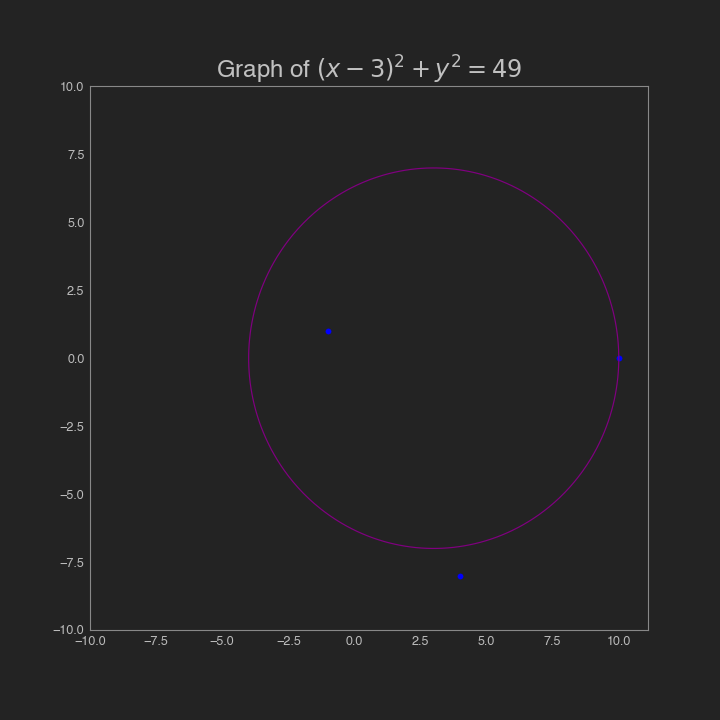
\includegraphics[width=1.0\columnwidth]{../q36/circle.png}
  \caption{Graph of Circle with Respective Point Locations}
\end{figure}
\end{center}


\end{document}
